\section{Глава 4. Графовые нейронные сети}
Графовые нейронные сети (Graph Neural Network - GNN) -- это методы глубокого обучения, основанные на графах. Как правило, они базируются на следующих фундаментальных аспектах: сверточных нейронных сетях (Convolutional Neural Network - CNN) и графовых эмбеддингах. 

Сверточные нейронные сети могут работать только с евклидовыми данными, такими как изображения (двумерная сетка) и эту структуру данных можно рассматривать как граф. Ключевыми принципами сверточных нейронных сетей являются: локальная связь, разделяемые веса и использование многослойности. И эти принципы могут иметь большое значение при решении задач в области графов, поскольку графы являются наиболее типичной локально связной структурой, а общие веса снижают вычислительные затраты. 

Главной проблемой для обобщения сверточных нейронных сетей на графы является то, что графы, как правило, в общем случае представляют собой нерегулярную неевклидову структуру данных (число узлов и связей между ними произвольно). Эту проблему и призвана решить графовая нейронная сеть, поскольку CNN не может должным образом обрабатывать ввод графа из-за того, что она обрабатывает  узлы в определенном порядке. Однако, в графе нет естественного порядка, поэтому, чтобы полностью представить граф, мы должны пройти через все возможные порядки узлов в качестве входных данных модели, которая будет очень избыточна при вычислениях. Для решения этой проблемы GNN распространяются на каждом узле соответственно, игнорируя порядок ввода узлов. Другими словами, вывод GNN является инвариантным для порядка ввода узлов. 

Другим важным аспектом является использование графовых эмбеддингов, которые учатся представлять узлы, ребра или подграфы графа в низкоразмерных векторах. Однако, использование методов графовых эмбеддингов имеет два серьезных недостатка. Во-первых, никакие параметры не разделяются между узлами при кодировании узлов в вектора, что приводит к неэффективности вычислений, поскольку это означает, что число параметров растет линейно с количеством узлов. Во-вторых, методы векторного представления, такие как DeepWalk и Node2Vec не имеют возможности обобщения, что означает, что они не могут иметь дело с динамическими графами или обобщаться на новые графы.

Поэтому на основе сверточных нейронных сетях и графовых эмбеддингов были введены графовые нейронные сети коллективно агрегирующие информацию из структуры графов, при это делая это вычислительно более эффективно.

\subsection{4.1. Оригинальная концепция графовой нейронной сети}

В задаче классификации узлов графа, каждый узел $v$, как правило, характеризуется вектором-признаков $x_v$ и меткой класса $t_v$, к которому принадлежит узел. Имея частично размеченный граф $G$,
целью графовой нейронной сети является изучение скрытого представления каждого узла $v$, т.е. $h_v \in \mathbb{R}^d$, зная информация о самом узле (признаки узла) и об окрестности узла. Полученное представление является $d$-мерным вектором и используется в дальнейшем для получения целевого значения $o_v$.  Более формально:
$$
h_v = f(x_v, x_{co[v]}, h_{ne[v]}, x_{ne[v]}) 
$$
где $x_v$ - признаки узла $v$, $x_{co[v]}$ - признаки ребер, соединенных с узлом $v$, $h_{ne[v]}$ - векторное представление узлов, находящихся в окрестности узла $v$, и $x_{ne[v]}$ - признаки узлов, находящихся в окрестности узла $v$.  Функция $f$ является функцией перехода, которая проецирует входные данные в $d$-мерное пространство. 

Уравнение выше представляется как итеративный процесс, используя Банахову теорему о неподвижной точке:
$$
H^{t+1} = F(H^t, X)
$$

$H$ и $X$ обозначают конкатенацию всех $h$ и $x$ соответственно.

Целевое значение графовой нейронной сети вычисляется путем передачи векторного представления $h_v$ и признаков $x_v$ в выходную функцию $g$:

$$
o_v = g(h_v, x_v)
$$
При этом, $f$ и $g$, могут быть интерпретированы как полносвязные нейронные сети прямого распространения. И параметры этих функций могут быть найдены как решение задачи минимизации функции потерь:
$$
	loss = \sum_{i=1}^p (t_i - o_i)
$$
которая может быть решена с помощью метода градиентного спуска.

Однако, оригинальный подход использования концепции графовой нейронной сети имеет существенные ограничения:
\begin{enumerate}
\item Она использует одни и те же параметры на итерации, в то время как большинство популярных нейронных сетей используют разные параметры в разных слоях.
\item Она не может обрабатывать информацию о ребрах (например, разные типы ребра в графе могут указывать на разные отношения между узлами)
\item Выбор эффективной функции, которая будет преобразовывать узлы в векторные представления.
\end{enumerate}

Поэтому для решения некоторых из этих проблем были предложены более улучшенные вариации исходной концепции графовой нейронной сети. 


\subsection{4.2. GraphSAGE}

Большинство существующих подходов векторного представления узлов графа являются трансдуктивными, т.е. они подходят только для графов с фиксированной структурой. Однако при добавлении новых узлов в граф трансдуктивные методы приходится полностью переучивать, что является вычислительно затратным и неэффективным способом для больших графов.

Метод GraphSAGE \cite{GraphSAGE } успешно решает вышеупомянутую проблему. Этот подход базируется на сверточных нейронных сетях, обобщая их от обработки простых решеток до произвольных графов. 

Ключевое отличие от трансдуктивных подходов является то, что вместо того, чтобы обучать векторное представление для каждого узла, мы обучаем набор агрегирующих функций, которые учатся собирать информацию о признаках из окрестности узла. При этом, каждая агрегирующая функция собирает информацию из окрестности, которая находится на определенном расстоянии от целевого узла. 

Более формально, процесс получения векторного представления узлов представлен в Алгоритме \ref{algo:2}:

\begin{algorithm}[H]
		\KwData{Граф $G(V,E)$; признаки узлов $x_v, \forall v \in V$; весовая матрица $W^k, \forall k \in \{1, 2, ..., K\}$; агрегирующие функции $AGGREGATE_k, \forall k \in \{1, 2, ..., K\}$; нелинейная функция активации $\sigma$}
		\KwResult{Векторное представление $z_v, \forall v \in V$ }
  $ h_v^0 = x_v, \forall v \in V$ \\
  \For{k=1...K}{
      \ForEach{$v \in V$}{
          $h_{N(v)}^k = AGGREGATE_k({h_u^{k-1}, \forall u \in N(v)})$ \\
          $h_v^k = \sigma(W^k \cdot CONCAT(h_v^{k-1}, h_{N(v)}^k));$
      }
      $h_v^k = \frac{h_v^k}{||h_v^k||_2}, \forall v \in V$
  }
  $z_v = h_v^K, \forall v \in V$

    \caption{Алгоритм генерации эмбеддингов GraphSAGE}
    \label{algo:2}
\end{algorithm}

Каждый агрегатор во внешнем цикле отвечает за обработку узлов, находящихся на глубине $k$ от исходного узла и при этом обрабатываются векторные представления узлов, полученные на предыдущем шаге. После того, как агрегатор заканчивает свою работу мы получаем вектор $h_{N(v)}^k$, который конкатенируется с векторным представлением текущего обрабатываемого узла $h_v^{k-1}$, которое получено на предыдущем шаге. Полученный вектор проходит через полно-связный слой с нелинейной функцией активации $\sigma$, на выходе которой получается новое векторное представление $h_v^k$, которое используется на следующем шаге цикла.
Стоит заметить, что на первой итерации агрегирующая функция $AGGREGATE_1$ в качестве эмбеддингов использует признаки узла $x_v$.  

Важным моментом является выбор агрегирующей функции и авторы исходной статьи говорят, что такая функция должна обладать свойством симметрии, поскольку это гарантирует, что наша модель нейронной сети может быть обучена и применена к произвольно упорядоченному набору узлов. В качестве агрегирующих функций может выбрана одна из следующих трех функций:
\begin{enumerate}
\item Mean агрегатор. Суть данного агрегатора заключается в том, что берется поэлементное среднее векторов.
\item LSTM агрератор. Данный агрегатор использует архитектуру, которая используется в нейронных сетях с долгой краткосрочной памятью, но поскольку данная архитектура не является симметричной, т.к. она обрабатывает фиксированную последовательность в определенном порядке, то при использовании данного метода применяется случайная перестановка.
\item Pooling агрегатор.  При таком подходе векторное представление каждого узла проходит через полно-связный слой нейронной сети и после этого преобразования применяется поэлементная операция max или mean пулинга.
\end{enumerate}

\subsection{4.3. Реализация графовой нейронной сети}

Архитектура нейронной сети GraphSAGE, описанная раннее, была реализована посредством языка программирования Python 3.6, а также  библиотек Keras \cite{keras} и StellarGraph \cite{stellargraph}. Выбор данного языка обусловлен тем, что он широко распространен в области машинного обучения и имеет в наличии множество библиотек для реализации нейронных сетей. 

В задачах предсказания возраста и пола пользователя архитектура нейронной сети состоит из 3 скрытых слоев и каждый слой преобразует поданный вектор признаков в 32-мерный эмбеддинг. При этом к каждому слою применен дропаут с вероятностью 0.5. Для решения задачи оптимизации выбран алгоритм RMSprop, а в качестве агрегатора - MeanAgregator.

В качестве выборки, которая подается на вход нейронной сети была выбрана выборка, к которой предварительно применены One Hot Encoding и стандартизация.


\begin{table}[b]
\centering
\begin{tabular}{|l|l|l|}
\hline
\multicolumn{1}{|c|}{\textbf{Метод}} & \multicolumn{1}{c|}{\textbf{MAE}}  \\ \hline
GraphSAGE                        &               4.7                                                              \\ \hline
\end{tabular}
\caption{Результаты работы метода GraphSAGE для определения возраста}
\label{graphsage age table}
\end{table}

\begin{table}[t]
\centering
\begin{tabular}{|l|l|l|l|l|l|}
\hline
\multicolumn{1}{|c|}{\textbf{Метод}} & \multicolumn{1}{c|}{\textbf{Accuracy}} & \multicolumn{1}{c|}{\textbf{Precision}} & \multicolumn{1}{c|}{\textbf{Recall}} & \multicolumn{1}{c|}{\textbf{F1}}  \\ \hline
GraphSAGE                       & 0.79                                        &           0.72                              &      0.92                                &     0.81                          \\ \hline

\end{tabular}
\caption{Результаты работы метода GraphSAGE для определения пола}
\label{graphsage gender table}
\end{table}

\begin{figure}[h!]
\begin{subfigure}[h]{0.5\linewidth}
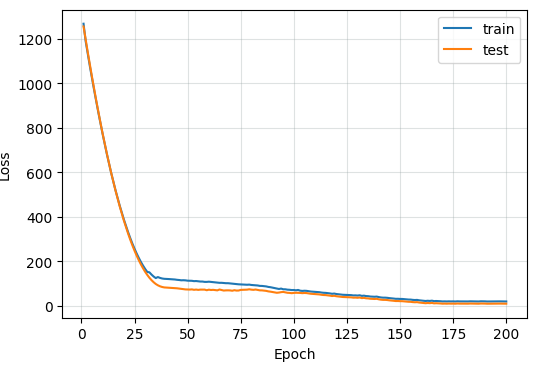
\includegraphics[width=\linewidth]{images/loss_age}
\caption{Loss}
\end{subfigure}
\hfill
\begin{subfigure}[h]{0.5\linewidth}
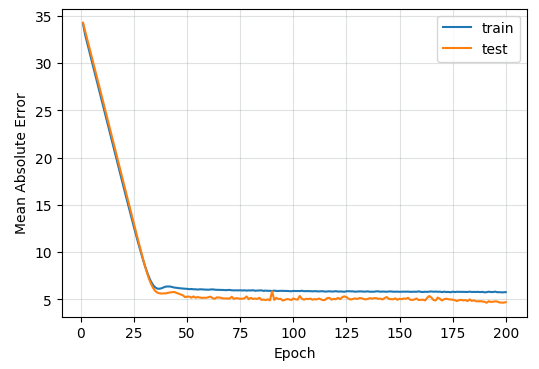
\includegraphics[width=\linewidth]{images/mae_age}
\caption{MAE}
\end{subfigure}%
\caption{Результаты алгоритма GraphSAGE в задаче определения возраста}
\label{fig:graphsage_age_results}
\end{figure}


\begin{figure}[h!]
\begin{subfigure}[h]{0.5\linewidth}
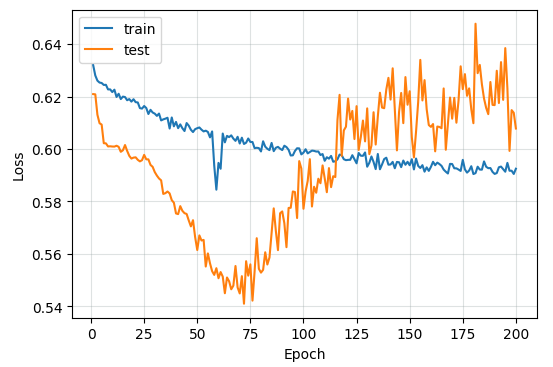
\includegraphics[width=\linewidth]{images/loss_gender}
\caption{Loss}
\end{subfigure}
\hfill
\begin{subfigure}[h]{0.5\linewidth}
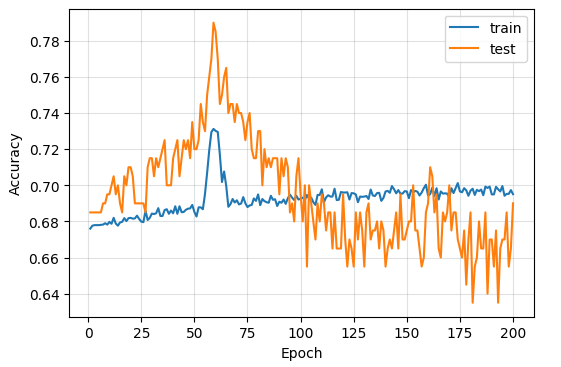
\includegraphics[width=\linewidth]{images/acc_gender}
\caption{Accuracy}
\end{subfigure}%
\caption{Результаты алгоритма GraphSAGE в задаче определения пола}
\label{fig:graphsage_gender_results}
\end{figure}

Полученные результаты можно наблюдать в Таблице \ref{graphsage age table} и в Таблице \ref{graphsage gender table}, а также процесс обучения отражен на Рис. \ref{fig:graphsage_age_results} и Рис. \ref{fig:graphsage_gender_results}. В задаче определения возраста нейронная сеть сработала хуже базовых алгоритмов машинного обучения, однако при определении возраста можно наблюдать неплохой прирост значений по всем метрикам, в особенности F1 меры.


По полученным графикам обучения можно сделать вывод, что оптимальное число эпох обучения в задаче определения пола находится в диапазоне от 50 до 75, а именно -- наилучшие результаты показала нейронная сеть при обучении на 59 эпохах. При этом использование большего числа эпох приводит к переобучению модели. Что касается задачи определения возраста, то после 30 эпохи идет незначительное улучшение качества алгоритма.

Стоит отметить, что обучение нейронной сети проходило как на CPU (на  8 ядерном процессоре Intel Scalable), так и на GPU (видеокарта NVIDIA TESLA K80). На CPU время обучения нейронной сети для задач определения возраста и пола заняло порядка 20000 секунд, в то время как на GPU  порядка 14000 секунд.   В целом можно наблюдать незначительный прирост в скорости обучения.



\clearpage


